\documentclass[a5paper]{article}
\usepackage{graphicx}
\usepackage{hyperref}
\usepackage[final]{pdfpages}
\usepackage[parfill]{parskip}% don't indent new sections
\usepackage[utf8]{inputenc}
\usepackage{listings}
\usepackage{listings-golang}
\usepackage{color}
\usepackage[a4paper]{geometry}
\pagestyle{empty}

\lstset{frame=tb,
    frame=single,
    aboveskip=3mm,
    belowskip=3mm,
    showstringspaces=false,
    columns=flexible,
    basicstyle={\small\ttfamily},
    numbers=left,
    keywordstyle=\color{red},
    stringstyle=\color{blue},
    commentstyle=\color{dkgreen},
    breaklines=true,
    breakatwhitespace=true,
    tabsize=4,
    language=Golang
}

\title{Applied Algorithms}
\author{Emil Lynegaard}

\begin{document}
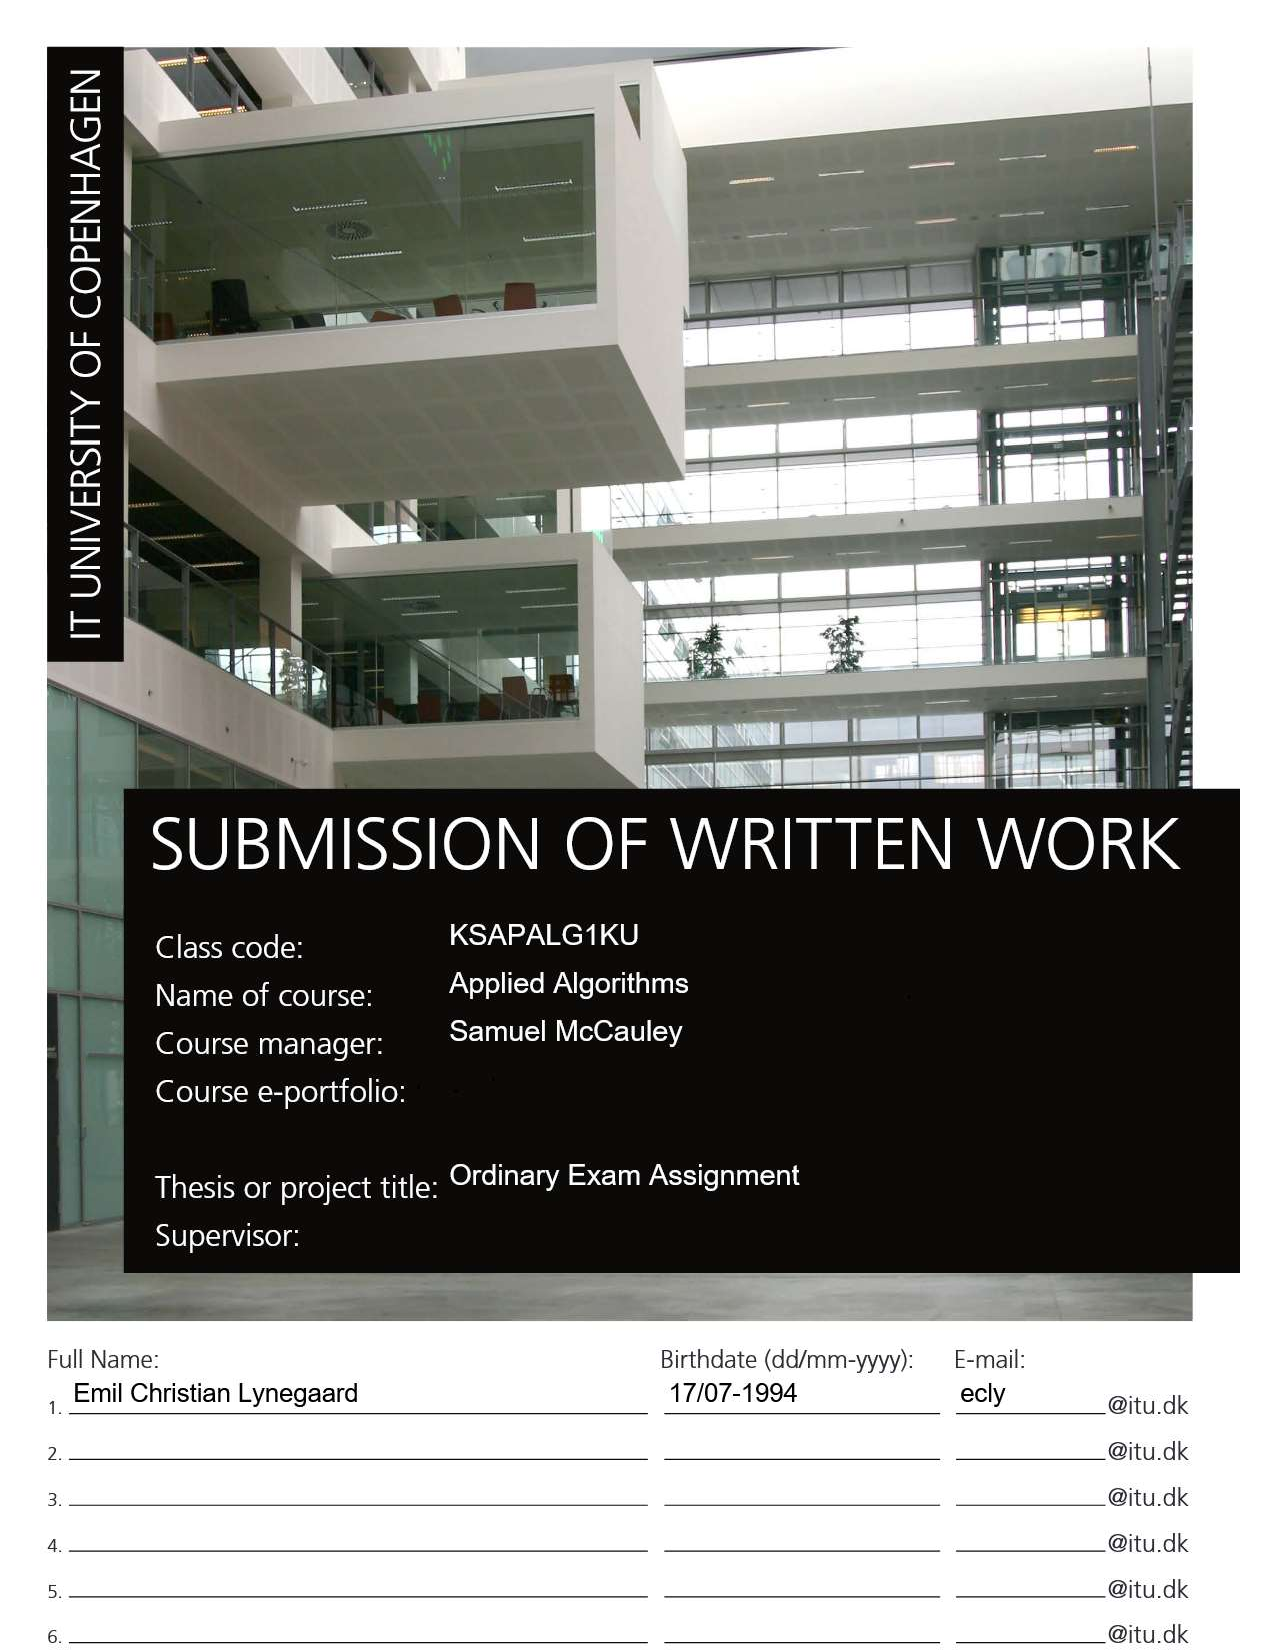
\includepdf[pages=1]{res/front_page.pdf}

\maketitle
\textit{I hereby declare that I have answered the exam questions myself without any outside help.}\\
\newpage

\newpage
\tableofcontents
\newpage

\section{Question 1}
\subsection{}

\begin{lstlisting}
package main

import "fmt"

func main() {
    fmt.Println("Hello World!")
}
\end{lstlisting}

% \begin{figure}[!ht]
%     \centering
%     \noindent\includegraphics[scale=0.5]{res/}
%     \caption{}
%     \label{fig:}
% \end{figure}

\section{Appendix}
%\subsection{SecComSys.java}\label{sec:akka}
%\lstinputlisting{../src/Erlang/SecComSys.java}
\end{document}
